\begin{enumerate}
  
\item A company produces two types of goods, $A$ and $B$, that require gold and
silver. Each unit of type $A$ requires $3g$ of silver and $1g$ of gold, while that of type $B$ requires $1g$ of silver and $2g$ of gold. The company can use at
the most $9g$ of silver and $8g$ of gold. If each unit of type $A$ brings a profit
of \rupee~120 and that of type $B$ \rupee~150, then find the number of units of each type that the company should produce to maximise profit. Formulate the above LPP and solve it graphically. Also, find the maximum profit.
\item Find the maximum value of $7x+6y$ subject to the constrains:
\begin{align}
	x+y &\geq   2\\
	2x+3y &\leq 6\\
	x \geq 0 \text{and} y &\geq 0
\end{align}
\item A window is in the form of a rectangular mounted by a semi-circular opening.The total perimeter of the window to admit maximum light through the whole opening.
\item Divide the number $8$ into two positive numbers such that the sum of the cube of one and the square of the other is maximum.
\item Find the maximum and the minimum values of 
\begin{align}
       z=5x+2y 
\end{align}	
		subject to the constrains:
\begin{align}
	-2x-3y &\leq -6\\
	x-2y &\leq 2\\
	6x+4y &\leq 24\\
	-3x+2y &\leq 3\\
	x \geq 0, y &\geq 0
\end{align}
 
 \item A furniture dealer deals in only two items : chairs and tables. He has \rupee~5,000  to invest and a space to store at most $60$ pieces. A table costs him \rupee~250 and a chair \rupee~50. He sells a table at a profit of \rupee~50 and a chair at
a profit of \rupee~ 15. Assuming that he can sell all the items he buys, how should he invest his money in order that he may maximize his profit ?
Formulate the above as a linear programming problem.
\item The least value of the function 
\begin{align}
	f(x)=2\cos(x) + x
\end{align}
		in the closed interval $\sbrak{0, \frac{\pi}{2}}$ is: 
\begin{enumerate}
    \item  $2$
    \item  $\frac{\pi}{6} + \sqrt{3}$
    \item  $\frac{\pi}{2}$
    \item The least value does not exist.
\end{enumerate}
\item A linear programming problem is as follows:
Minimize 
\begin{align}
	Z=30x+50y 
\end{align}
		subject to the constrains,
\begin{align}
	3x+5y &\geq 15\\
	2x+3y &\leq 18\\
	x \geq 0, y &\geq 0
\end{align}
In the feasible region, the minimum value of $Z$ occurs at 
\begin{enumerate}
    \item a unique point 
    \item no point
    \item infinitely many points 
    \item two points only
\end{enumerate}
\item The area of a trapezium is defined by function $f$
and given by 
\begin{align}
	f(x)=(10+x)\sqrt{100-x^2}
\end{align}
			, then the area when it is maximised is:
\begin{enumerate}
    \item $75cm^2$
    \item $7\sqrt{3}cm^2$
    \item $75\sqrt{3}cm^2$
    \item $5cm^2$
\end{enumerate}
\item For an objective function 
\begin{align}
	Z=ax+by
\end{align}		
		,where $a,b>0$;the corner points of the feasible region determined by a set of constrains (linear inequalities) are $(0,20)$, $(10,10)$, $(30,30)$, and $(0,40)$.The condition on $a$ and $b$ such that the maximum $Z$ occurs at the points $(30,30)$ and $(0,40)$ is: 
\begin{enumerate}
    \item $b-3a=0$
    \item $a=3b$
    \item $a+2b=0$
    \item $2a-b=0$
\end{enumerate}
\item In a linear programming problem, the constrains on the decision variables $x$ and $y$ are $x-3y \geq 0, y \geq 0, 0\leq x \leq 3$.The feasible region 
\begin{enumerate}
    \item is not in the first quadrant
    \item is bounded in the first quadrant 
    \item is unbounded in the first quadrant 
    \item does not exist  
\end{enumerate}
\item Based on the given shaded region in figure \ref{fig:19/2021/041} as the feasible region in the graph, at which point(S) is the objective function 
\begin{align}
	Z=3x+9y 
\end{align}
		maximum?
\begin{figure}[h]
    \centering{}
    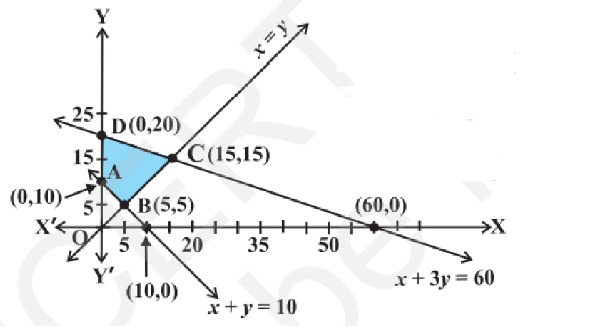
\includegraphics[width=\columnwidth]{figs/opti-21-fig1.jpg}
	\caption{Optimization graph}
    \label{fig:19/2021/041}
\end{figure}
\begin{enumerate}
    \item point $B$
    \item point $C$
    \item point $D$
    \item every point on the line segment $CD$   
\end{enumerate}
\item In figure \ref{fig:23/2021/041}, the feasible region for a LPP is shaded.The objective function 
\begin{align}
	Z=2x-3y
\end{align}
		,will be minimum at:
\begin{figure}[h]
    \centering{}
     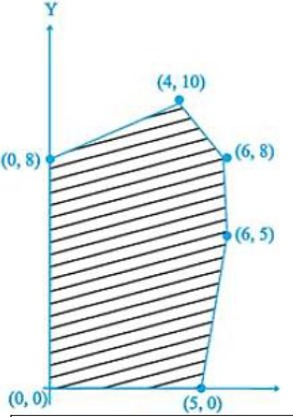
\includegraphics[width=\columnwidth]{figs/opti-21-fig2.jpg}
	\caption{Optimization graph}
     \label{fig:23/2021/041}                       
\end{figure}
\begin{enumerate}
    \item $(4,10)$
    \item $(6,8)$
    \item $(0,8)$
    \item $(6,5)$
\end{enumerate}
    
\end{enumerate}
